\documentclass[11pt]{scrartcl}
\usepackage{graphicx}
\graphicspath{{./}}
\usepackage[sexy]{evan}
\usepackage[normalem]{ulem}
\usepackage{hyperref}
\usepackage{mathtools}
\hypersetup{
    colorlinks=true,
    linkcolor=blue,
    filecolor=magenta,      
    urlcolor=cyan,
    pdfpagemode=FullScreen,
    }
\usepackage[most]{tcolorbox}
\renewcommand{\dangle}{\measuredangle}

\renewcommand{\baselinestretch}{1.5}

\addtolength{\oddsidemargin}{-0.4in}
\addtolength{\evensidemargin}{-0.4in}
\addtolength{\textwidth}{0.8in}
% \addtolength{\topmargin}{-0.2in}
% \addtolength{\textheight}{1in} 


\setlength{\parindent}{0pt}

\usepackage{pgfplots}
\pgfplotsset{compat=1.15}
\usepackage{mathrsfs}
\usetikzlibrary{arrows}

\title{2024 Asia International Mathematical Olympiad Open Trial Simulation 2}
\author{Question Paper}
\date{17.00, 1 May 2024 - 18.30, 3 May 2024}

\begin{document}
\maketitle
\begin{center}
    \Huge
    \boxed{\textbf{Grade 3 - 4}}
\end{center}
\vspace{3cm}

\begin{flushright}
    \huge
   Time allowed: 90 minutes
\end{flushright}

\vspace{3cm}
\normalsize
Write down the answer according to the instruction given in questions. \textbf{The calculation result are guaranteed in the integers form.} If the answer is in surd form, represent the answer which is in the simplest form. \textbf{No need to write down any unit.}

\vspace{2cm}
Link to submit the answers: \url{https://forms.gle/mucWuTaanZhq814k8}



\pagestyle{plain}
\newpage
Section A – each question carries 4 marks

\hrulefill %linefill
\begin{enumerate}
    \item Find the sum of all positive factors of 42.
    \vspace{10cm} \item 42 trees are planted along a road from one end to another on both sides. Every two adjacent trees are 8 metres apart. How long is the road in metres?
    \vspace{10cm} \item The number $202431122024311220243112\ldots$ is written on and on. What is the $90^{th}$ digit?
    \vspace{13cm} \item Evaluate the value of $3 \times (2024^2 - 2^2) \div (2022 \times 2026)$.
    \vspace{10cm} \item Find the remainder when $202420242024\ldots2024$ (with 2024 "2024"'s) is divided by 9. 
    \vspace{13cm} \item The ages of Mickey and Chesney add up to 95. The age of Mickey is 25 more than 4 times that of Chesney. Find the age of Mickey.
    \vspace{10cm} \item Find the perimeter of the figure if all angles in the figure are right angles. 
    \begin{figure}[h]
        \centering
        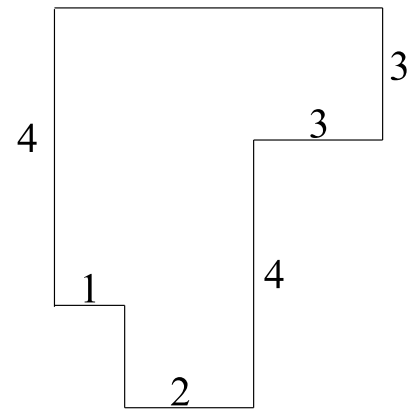
\includegraphics[width=0.4\textwidth]{StarGen/AIMO Trial G3-4 2024/perim.png}
    \end{figure}
    \vspace{8cm} \item 6 different three-digit numbers can be formed using the digits "3", "6" and "8". Find the sum of these 6 three-digit numbers.
\end{enumerate}

\newpage
Section B – each question carries 5 marks

\hrulefill %linefill
\begin{enumerate}[resume]
    \item Among the 36 natural numbers from 1 to 36, at least how many numbers have to be picked so that there must be 2 numbers whose difference is 18?
    
    \vspace{10cm} \item Define the operation symbol $\oplus$ following this pattern:
    \begin{align*}
    1 \oplus 5 &= 1 - 2 + 3 - 4 + 5\\
    3 \oplus 8 &= 3 - 4 + 5 - 6 + 7 - 8\\
    5 \oplus 9 &= 5 - 6 + 7 - 8 + 9\\
    \dots& \text{(and so on ...)}
    \end{align*}
    Find the value of $(5 \oplus 10) - (4 \oplus 9).$
    
    \vspace{10cm} \item Ronny runs after Sunny at a speed of 25 km/h. In the beginning, Sunny is 3 km ahead of Ronny. If Ronny manages to meet Sunny 12 minutes later, how many kilometres does Sunny run each hour?
    
    \vspace{13cm} \item Define $F(a)$ as $3 \times a+1$. Find the value of $n$ if $F(F(n))=40$.
    
    \vspace{10cm} \item 5 bags of rice, 6 bags of soybeans and 9 bags of red beans weigh 60 kilograms, while 17 bags of rice, 18 bags of soybean and 27 bags of red beans weigh 200 kilograms. So how many kilograms does 1 bag of rice weigh?
    
    \vspace{10cm} \item There are two positive integers. Their sum is 143 and their product is 1080. Find the greater number among these two numbers.
    
    \vspace{10cm} \item The four members in Mandy's family have their ages add up to 99. Her brother is 8 years younger than Mandy. Dad is 3 years older than Mum. 10 years ago, the family ages added up to 65. How old is Mum this year?
    
    \vspace{10cm} \item Evaluate $20^2-18^2+16^2-14^2+\dots+4^2-2^2$.
\end{enumerate}

\newpage
Section C – each question carries 7 marks

\hrulefill %linefill
\begin{enumerate}[resume]
    \item The larger rectangle in the figure is formed by 5 identical smaller rectangles. If the perimeter of the larger rectangle is $52$cm. Find the perimeter of a small rectangle. 
    \begin{figure}[h]
        \centering
        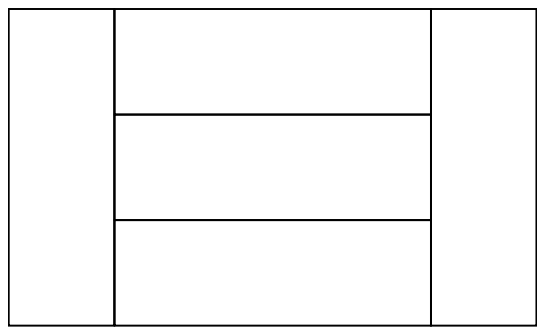
\includegraphics[width=0.4\textwidth]{StarGen/AIMO Trial G3-4 2024/5rect2.png}
    \end{figure}
    
    \vspace{8cm} \item A Hacker enters the password "394052186" when he comes to a system of computers. The system says they have swapped two of the numbers. How many passwords at most does the Hacker need to enter more?

    \vspace{10cm} \item There are 55 cards. "1" is written on 1 card, "2" on 2 cards, "3" on 3 cards, \ldots, "10" on 10 cards. Now several cards are picked so that the sum of the numbers on all cards is 312. How many cards can be picked at most?
    
    \vspace{8cm} \item The figure shows some numbered squares. If squares are to be tiled up to 2024 following the pattern, find the number in the square which is just above 127. 
    \begin{figure}[h]
        \centering
        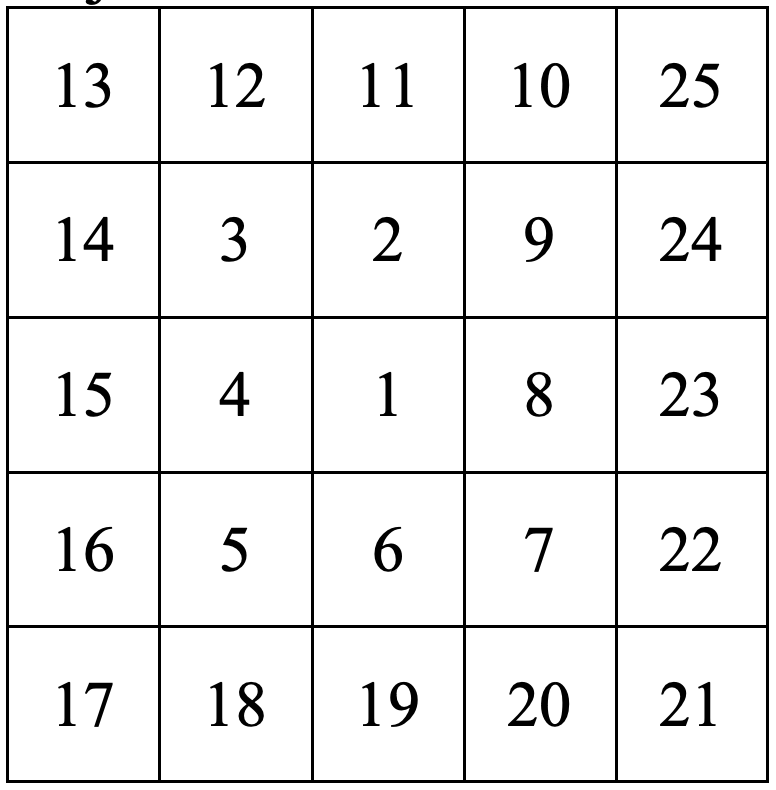
\includegraphics[width=0.4\textwidth]{StarGen/AIMO Trial G3-4 2024/square-siput.png}
    \end{figure}
\end{enumerate}

\end{document}